\section{Quotient Groups and Homomorphisms}

\subsection{Definitions and Examples}

Let $G$ and $H$ be groups.

\begin{problems}
    \item Let $\phi : G \to H$ be a homomorphism and let $E$ be a subgroup of $H$. Prove that $\phi\inv(E) \leq G$ (i.e., the preimage or pullback of a subgroup under a homomorphism is a subgroup). If $E \nsub H$ prove that $\phi\inv(E) \nsub G$. Deduce that $\ker(\phi) \nsub G$.
    \begin{sol}
        Since $E \leq H$, then $1_H \in E$. Since $\phi(1_G) = 1_H \in E$, then $1_G \in \phi\inv(E)$ so that it is nonempty. Suppose $x, y \in \phi\inv(E)$. Then $\phi(x), \phi(y) \in E$ so that $\phi(x)\phi(y)\inv = \phi(xy\inv) \in E$. Then $xy\inv \in \phi\inv(E)$, hence $\phi\inv(E) \leq G$.
        
        If $E \nsub H$, then $heh\inv \in E$ for every $e \in E$ and $h \in H$. Let $x \in \phi\inv(E)$ and $g \in G$. Note that $\phi(g) \in H$. Then
        \[\phi(g)\phi(x)\phi(g)\inv = \phi(gxg\inv) \in E\]
        so that $gxg\inv \in \phi\inv(E)$. Then $\phi\inv(E) \nsub G$, and since $\ker(\phi) = \phi\inv(1_H)$, then $\ker(\phi) \nsub G$ as well.
    \end{sol}
    \item Let $\varphi : G \to H$ be a homomorphism of groups with kernel $K$ and let $a,b \in \varphi(G)$. Let $X \in G/K$ be the fiber above $a$ and let $Y$ be the fiber above $b$, i.e.,
    $X = \varphi^{-1}(a)$, $Y = \varphi^{-1}(b)$. Fix an element $u \in X$ (so $\varphi(u)=a$). Prove that if $XY = Z$ in the quotient group $G/K$ and $w$ is any member of $Z$, then there is some $v \in Y$ such that $uv = w$. [Show $u^{-1}w \in Y$.]
    \begin{sol}
        To show that $v = u\inv w \in Y$, then
        \[\phi(v) = \phi(u\inv w) = \phi(u)\inv \phi(w) = a\inv (ab) = b \in Y \qh\]
    \end{sol}
    \item Let $A$ be an abelian group and let $B$ be a subgroup of $A$.
    Prove that $A/B$ is abelian. Give an example of a non-abelian group $G$ containing a proper normal subgroup $N$ such that $G/N$ is abelian.
    \begin{sol}
        Let $aB, a'B \in A/B$. Then
        \[(aB)(a'B) = (aa')B = (a'a)B = (a'B)(aB)\]
        so that $A/B$ is abelian.

        To produce an abelian quotient group from a non-abelian group, a good thought is to consider the centers of non-abelian groups. In this case, we may choose $G = D_8$ with $Z(D_8) = \gen{r^2} \nsub D_8$. Since $D_8/\gen{r^2} \cong V_4$, then the quotient group is abelian.
    \end{sol}
    \item Prove that in the quotient group $G/N$, $(gN)^{\alpha} = g^{\alpha}N$ for all $\alpha \in \mathbb{Z}$.
    \begin{sol}
        Note that $(gN)^0 = 1N = g^0N$, and $(gN)\inv = g\inv N$ by \autoref{prop3.5}. It suffices to show that the relationship holds for $\alpha \in \zp$. To that end, note that $\alpha = 1$ holds. Supposing it holds for some $\alpha$, then
        \[(gN)^{\alpha + 1} = (gN)^\alpha (gN) = (g^\alpha N)(gN) = g^{\alpha + 1}N\]
        so that the result is true by induction.
    \end{sol}
    \item Use the preceding exercise to prove that the order of the element $gN$ in $G/N$ is $n$, where $n$ is the smallest positive integer such that $g^n \in N$ (and $gN$ has infinite order if no such positive integer exists). Give an example to show that the order of $gN$ in $G/N$ may be strictly smaller than the order of $g$ in $G$.
    \begin{sol}
        Let $gN \in G/N$. If possible, let $n \in \zp$ be the smallest integer such that $g^n \in N$. Then $g^nN = (gN)^n = 1N$ so that $|gN| \leq n$. Moreover, if $m \in \zp$ is an integer such that $(gN)^m = 1N$, then $g^mN = 1N$ so that $g^m \in N$. By minimality of $n$, then $|gN| \geq n$ so that $|gN| = n$.

        If there is no such $n$, then $g^k \not\in N$ for every $k \in \zp$. Suppose for contradiction that $gN$ has infinite order $x$. Then $(gN)^x = g^xN = 1N$, or that $g^x \in N$, contradicting our previous assumption. It follows that $gN$ has infinite order. Moreover, let $G$ be a nontrivial group with nonidentity $g \in G$. Noting that $G \nsub G$, then $gG \in G/N$ has order 1, but $\abs g > 1$.
    \end{sol}
    \item Define $\varphi : \mathbb{R}^{\times} \to \{\pm 1\}$ by letting $\varphi(x)$ be $x$ divided by the absolute value of $x$. Describe the fibers of $\varphi$ and prove that $\varphi$ is a homomorphism.
    \begin{sol}
        The fibers of $\phi$ are as follows: the positive reals map to 1, and the negative reals map to $-1$. Moreover, for any $x, y \in \r\unt$, then
        \[\phi(xy) = \frac{xy}{\abs{xy}} = \frac{x}{\abs x} \cdot \frac{y}{\abs y} = \phi(x)\phi(y) \qh\]
    \end{sol}
    \item Define $\pi : \mathbb{R}^2 \to \mathbb{R}$ by $\pi((x,y)) = x + y$. Prove that $\pi$ is a surjective homomorphism and describe the kernel and fibers of $\pi$ geometrically.
    \begin{sol}
        Let $(x, y), (a, b) \in \r^2$. Then
        \begin{align*}
            \pi((x, y) + (a, b)) & = \pi((x + a, y + b)) \\
            & = (x + a) + (y + b) \\
            & = (x + y) + (a + b) \\
            & = \pi((x, y)) + \pi((a, b))
        \end{align*}
        so that $\pi$ is a homomorphism. Moreover, for any $a \in \r$, then $\pi((a, 0)) = a$ so that $\pi$ is surjective. $\ker(\pi)$ is the diagonal line in $\r$ with equation $y = -x$, and the fiber $\phi\inv(a)$ for any $a \in \r$ is the diagonal line $y = -x + a$, or just a vertical translation of the kernel.
    \end{sol}
    \item Let $\varphi : \mathbb{R}^{\times} \to \mathbb{R}^{\times}$ be the map sending $x$ to the absolute value of $x$. Prove that $\varphi$ is a homomorphism and find the image of $\varphi$. Describe the kernel and the fibers of $\varphi$.
    \begin{sol}
        Let $x, y \in \r\unt$. Then
        \[\phi(xy) = |xy| = |x||y| = \phi(x)\pi(y)\]
        so that $\phi$ is a homomorphism. Moreover, $\phi(\pm a) = a$ for any $a \in \r^+$ so that $\im(\phi)$ is the positive reals. $\ker(\phi) = \set{1, -1}$ since no other real number has an absolute value of 1, and the fiber of $\phi$ over $a$ is the pair of reals $\{a, -a\}$.
    \end{sol}
    \item Define $\varphi : \mathbb{C}^{\times} \to \mathbb{R}^{\times}$ by $\varphi(a+bi) = a^2 + b^2$. Prove that $\varphi$ is a homomorphism and find the image of $\varphi$. Describe the kernel and the fibers of $\varphi$ geometrically (as subsets of the plane).
    \begin{sol}
        Let $a + bi, c + di \in \c\unt$. Then
        \begin{align*}
            \phi((a + bi)(c + di)) & = \phi((ac - bd) + (ad + bc)i) \\
            & = (ac - bd)^2 + (ad + bc)^2 \\
            & = a^2c^2 - 2abcd + b^2d^2 + a^2d^2 + 2abcd + b^2c^2 \\
            & = c^2(a^2 + b^2) + d^2(a^2 + b^2) \\
            & = (a^2 + b^2)(c^2 + d^2) \\
            & = \phi(a + bi)\phi(c + di)
        \end{align*}
        and $\phi$ is a homomorphism. Note that $a^2 + b^2 > 0$ for any $a, b$ where at least one of them is nonzero, so $\im(\phi) \subseteq \r^+$. Also, $\phi(\sqrt a + 0i) = a$ for any $a \in \r^+$, so $\im(\phi) = \r^+$. $\ker(\phi) = \{a + bi \in \c\unt \mid a^2 + b^2 = 1\}$ is simply the circle of radius 1, and the fiber of $\phi$ over some $a \in \r\unt$ is the circle with radius $\sqrt a$.
    \end{sol}
    \item Let $\phi : \intmod[8] \to \intmod[4]$ by $\phi(\bar  a) = \bar  a$. Show that this is a well defined, surjective homomorphism and describe its fibers and kernel explicitly (showing that $\phi$ is well defined involves the fact that $\bar  a$ has a different meaning in the domain and range of $\phi$).
    \begin{sol}
        Suppose $\bar  a = \bar  b$ for $\bar  a, \bar  b \in \intmod[8]$. Then $a = b + 8k$ for $k \in \z$, and
        \[\phi(\bar  a) = \bar  a = \bar{b + 8k} = \bar{b + 4(2k)} = \bar  b = \phi(\bar  b)\]
        Moreover, this is a homomorphism as
        \[\phi(\bar  a + \bar  b) = \phi(\bar{a + b}) = \bar{a + b} = \bar  a + \bar  b = \phi(\bar  a) + \phi(\bar  b)\]
        and is clearly surjective as $\phi(\bar  a) = \bar  a$ for any $\bar  a \in \intmod[4]$. The fibers are the following, noting that $\ker(\phi) = \phi\inv(\bar  0)$:
        \begin{align*}
            \phi\inv(\bar  0) & = \set{\bar  0, \bar  4} \\
            \phi\inv(\bar  1) & = \set{\bar  1, \bar  5} \\
            \phi\inv(\bar  2) & = \set{\bar  2, \bar  6} \\
            \phi\inv(\bar  3) & = \set{\bar  3, \bar  7} \qh
        \end{align*}
    \end{sol}
    \item Let $F$ be a field and let
    \[G = \set*{\left.
    \begin{pmatrix}
        a & b \\
        0 & c 
    \end{pmatrix}~\right|~a, b, c \in F, ac \neq 0} \leq \gl_2(F)\]
    \begin{problems}
        \item Prove that the map
        \[\phi : 
        \begin{pmatrix}
            a & b \\
            0 & c
        \end{pmatrix} \mapsto a\]
        is a surjective homomorphism from $G$ onto $F\unt$ (recall that $F\unt$ is the multiplicative group of nonzero elements in $F$). Describe the fibers and kernel of $\phi$.
        \item Prove that the map
        \[\psi : 
        \begin{pmatrix}
            a & b \\
            0 & c
        \end{pmatrix} \mapsto (a, c)\]
        is a surjective homomorphism from $G$ onto $F\unt \times F\unt$. Describe the fibers and kernel of $\psi$. 
        \item Let
        \[H = \set*{\left .
        \begin{pmatrix}
            1 & b \\
            0 & 1
        \end{pmatrix} ~\right\vert~b \in F}\]
        Prove that $H$ is isomorphic to the additive group $F$.
    \end{problems}
    \begin{solalph}
        \item Note that
        \[\phi\left(
        \begin{pmatrix}
            a & 1 \\
            0 & 1
        \end{pmatrix}\right) = a\]
        so that $\phi$ is surjective. Moreover, for any $a, b, c, d, e, f \in F$ with $ac \neq 0$ and $df \neq 0$, we have
        \[\phi\left(
        \begin{pmatrix}
            a & b \\
            0 & c
        \end{pmatrix}
        \begin{pmatrix}
            d & e \\
            0 & f
        \end{pmatrix}\right) = 
        \phi\left(
        \begin{pmatrix}
            ad & ae + bf \\
            0 & cf
        \end{pmatrix}\right) = ad = 
        \phi\left(
        \begin{pmatrix}
            a & b \\
            0 & c
        \end{pmatrix}\right)
        \phi\left(
        \begin{pmatrix}
            d & e \\
            0 & f
        \end{pmatrix}\right)\]
        and $\phi$ is then a homomorphism. The fiber of $a \in F\unt$ over $\phi$ is
        \[\phi\inv(a) = 
        \set*{\left.
        \begin{pmatrix}
            a & s \\
            0 & t
        \end{pmatrix}~\right|~s, t \in F, t \neq 0}\]
        with $\ker(\phi) = \phi\inv(1)$.
        \item Showing that $\psi$ is a surjective homomorphism is very similar to the previous part. The fiber of any $(a, c) \in F\unt \times F\unt$ is
        \[\psi\inv((a, c)) = 
        \set*{\left.
        \begin{pmatrix}
            a & s \\
            0 & c
        \end{pmatrix}~\right|~s \in F}\]
        with $\ker(\psi) = \psi\inv((1, 1))$.
        \item Define the mapping $\pi : H \to F$ given by
        \[\pi\left(
        \begin{pmatrix}
            1 & b \\
            0 & 1
        \end{pmatrix}\right) = b\]
        Then its inverse $\pi\inv : F \to H$ given by
        \[\pi\inv(b) = 
        \begin{pmatrix}
            1 & b \\
            0 & 1
        \end{pmatrix}\]
        is a two-sided inverse of $\pi$ so that $\pi$ is a bijection. Moreover, for $b, c \in F$, then
        \[\pi\left(
        \begin{pmatrix}
            1 & b \\
            0 & 1
        \end{pmatrix}
        \begin{pmatrix}
            1 & c \\
            0 & 1
        \end{pmatrix}\right) = 
        \pi\left(
        \begin{pmatrix}
            1 & b + c \\
            0 & 1
        \end{pmatrix}\right) = b + c = 
        \pi\left(
        \begin{pmatrix}
            1 & b \\
            0 & 1
        \end{pmatrix}\right) + 
        \pi\left(
        \begin{pmatrix}
            1 & c \\
            0 & 1
        \end{pmatrix}\right)\]
        so that $\pi$ is a homomorphism. Then $\pi$ is an isomorphism, and $H \cong F$.
    \end{solalph}
    \item Let $G$ be the additive group of real numbers, let $H$ be the multiplicative group of complex numbers of absolute value $1$ (the unit circle $S^1$ in the complex plane) and let $\varphi : G \to H$ be the homomorphism $\varphi : r \mapsto e^{2\pi i r}$. Draw the points on a real line which lie in the kernel of $\varphi$. Describe similarly the elements in the fibers of $\varphi$ above the points $-1$, $i$, and $e^{4\pi i/3}$ of $H$.
    \begin{sol}
        Since $e^{2\pi ir} = 1$ if and only if $r$ is an integer, then $\ker(\phi) = \z$. On a number line, this is shown as
        \begin{center}
            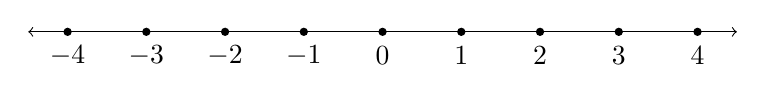
\begin{tikzpicture}
                \draw[<->] (-4.5, 0) -- (4.5, 0);
    
                \foreach \x in {-4, -3, -2, -1, 0, 1, 2, 3, 4}
                    \fill (\x, 0) circle (1.5pt);

                \foreach \x in {-4, -3, -2, -1, 0, 1, 2, 3, 4}
                    \node at (\x, -0.3) {$\x$};
            \end{tikzpicture}
        \end{center}
        Moreover, note that $-1 = e^{-2\pi i/2}$ and $i = e^{2\pi i/4}$. Then the fibers of these elements are just the integral differences of $1/2, 1/4$, and $2/3$ respectively, since $4\pi i/3 = 2/3(2\pi i)$:
        \begin{align*}
            \phi\inv(-1) & = \frac 12 + \z = \set*{\left.\frac 12 + n~\right|~n \in \z} \\
            \phi\inv(i) & = \frac 14 + \z = \set*{\left.\frac 14 + n~\right|~n \in \z} \\
            \phi\inv(e^{4\pi i/3}) & = \frac 23 + \z = \set*{\left.\frac 23 + n~\right|~n \in \z} \qh
        \end{align*}
    \end{sol}
    \item Repeat the preceding exercise with the map $\varphi$ replaced by the map $\varphi : r \mapsto e^{4\pi i r}$.
    \begin{sol}
        The kernel of $\phi$ is $\frac12\z$, or
        \begin{center}
            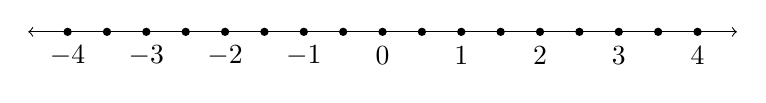
\begin{tikzpicture}
                \draw[<->] (-4.5, 0) -- (4.5, 0);
    
                \foreach \x in {-4, -3.5, -3, -2.5, -2, -1.5, -1, -0.5, 0, 0.5, 1, 1.5, 2, 2.5, 3, 3.5, 4}
                    \fill (\x, 0) circle (1.5pt);

                \foreach \x in {-4, -3, -2, -1, 0, 1, 2, 3, 4}
                    \node at (\x, -0.3) {$\x$};
            \end{tikzpicture}
        \end{center}
        Moreover, the fibers are just all halved, so
        \begin{align*}
            \phi\inv(-1) & = \frac14 + \frac12 \z = \set*{\left.\frac14 + \frac n2~\right|~n \in \z} \\
            \phi\inv(-i) & = \frac18 + \frac12 \z = \set*{\left.\frac18 + \frac n2~\right|~n \in \z} \\
            \phi\inv(e^{4\pi i/3}) & = \frac13 + \frac12 \z = \set*{\left.\frac13 + \frac n2~\right|~n \in \z} \qh
        \end{align*}
    \end{sol}
    \item Consider the additive quotient group $\mathbb{Q}/\mathbb{Z}$.
    \begin{problems}
        \item Show that every coset of $\mathbb{Z}$ in $\mathbb{Q}$ contains exactly one representative $q \in \mathbb{Q}$ in the range $0 \le q < 1$.
        \item Show that every element of $\mathbb{Q}/\mathbb{Z}$ has finite order but that there are elements of arbitrarily large order.
        \item Show that $\mathbb{Q}/\mathbb{Z}$ is the torsion subgroup of $\mathbb{R}/\mathbb{Z}$ (cf.\ Exercise 6, Section 2.1).
        \item Prove that $\mathbb{Q}/\mathbb{Z}$ is isomorphic to the multiplicative group of roots of unity in $\mathbb{C}^\times$.
    \end{problems}
    \begin{solalph}
        \item Suppose $t \in \q$, and put $t = a/b$ in lowest terms. Then there exists unique $q, r$ such that $a = bq + r$, or that $t = q + r/b$, where $0 \leq r < 1$. Then $t + \z = q + r/b + \z = r/b + \z$. Since $r$ is unique, then $r/b$ is the representative of $t + \z$ such that $0 \leq r < 1$.
        \item Suppose $t = p/q \in \q$. Then $|t + \z| \leq q$, since $q(t + \z) = qt + \z = \z$ so that $t + \z$ has finite order. Moreover, $1/k + \z \in \q/\z$ has order $k$, but because $k \in \z$ can be made arbitrarily large, then $1/k + \z$ has arbitrarily large order.
        \item Note that $\q/\z \subseteq \tor(\r/\z)$ by the previous exercise, so it remains to show that cosets with irrational representatives do not have finite order. If $x + \z \in \r/\z$ with finite order $n$, and $x \in \r - \q$, then $n(x + \z) = nx + \z = \z$ implies that $nx \in \z$. But since $n \in \zp$, this implies that $x \in \z$, contradicting that it was irrational. Hence, $\tor(\r/\z) = \q/\z$.
        \item By Exercise 3.1.12, we have $\r/\z \cong S^1$. Note that $\tor(S^1)$ consists of $z \in \c\unt$ such that $z^n = 1$, which is precisely the set of roots of unity. Since $\tor(\r/\z) = \q/\z$, then $\q/\z$ is isomorphic to the set of roots of unity.
    \end{solalph}
    \item Prove that a quotient of a divisible abelian group by any proper subgroup is also divisible. Deduce that $\mathbb{Q}/\mathbb{Z}$ is divisible (cf.\ Exercise 19, Section 2.4).
    \begin{sol}
        Let $A$ be a divisible abelian group, and let $B$ be a proper subgroup of $A$. Pick $aB \in A/B$. Since $A$ is divisible, there exists $x \in A$ such that $x^n = a$ for $x \in A$ and $n \in \z$. Then $(xB)^n = x^nB = aB$ so that $A/B$ is divisible. Since $\q$ is divisible, and $\z < \q$ is proper, then $\q/\z$ is also divisible.
    \end{sol}
    \item Let $G$ be a group, let $N$ be a normal subgroup of $G$, and let $\bar{G} = G/N$. Prove that if $G = \langle x, y \rangle$ then $\bar{G} = \langle \bar{x}, \bar{y} \rangle$. Prove more generally that if $G = \langle S \rangle$ for any subset $S$ of $G$, then $\bar{G} = \langle \bar{S} \rangle$.
    \begin{sol}
        If $G = \gen S$, then for every $g \in G$, we have
        \[g = s_1s_2 \dots s_n \quad \text{where $s_i \in S$ for $1 \le i \le n$}\]
        Let $\bar S = \{sN \mid s \in S\}$. Then for any $\bar g \in \bar G$, we have
        \[gN = (s_1s_2 \ldots s_n)N = (s_1N)(s_2N) \dots (s_nN)\]
        so that $\bar g \in \bar S$. Hence, $\bar G = \gen{\bar S}$. The case where $\bar G = \gen{\bar x, \bar y}$ is similar, where every element $g \in G$ is of the form $g = w(x, y)$, where $w(x, y)$ denotes a word in $\gen{x, y}$.
    \end{sol}
    \item Let $G$ be the dihedral group of order $16$ (whose lattice appears in Section 2.5): $G = \langle r,s \mid r^8 = s^2 = 1,\ rs = sr^{-1} \rangle$, and let $\bar{G} = G/\langle r^4 \rangle$ be the quotient of $G$ by the subgroup generated by $r^4$ (this subgroup is the center of $G$, hence is normal).
    \begin{problems}
        \item Show that the order of $\bar{G}$ is $8$.
        \item Exhibit each element of $\bar{G}$ in the form $\bar{s}^a \bar{r}^b$, for some integers $a$ and $b$.
        \item Find the order of each of the elements of $\bar{G}$ exhibited in (b).
        \item Write each of the following elements of $\bar{G}$ in the form $\bar{s}^a \bar{r}^b$, for some integers $a$ and $b$ as in (b): $\bar{rs}$, $\bar{sr^{-2}s}$, $\bar{s^{-1}r^{-1}sr}$.
        \item Prove that $\bar{H} = \langle \bar{s}, \bar{r}^2 \rangle$ is a normal subgroup of $\bar{G}$ and $\bar{H}$ is isomorphic to the Klein $4$-group. Describe the isomorphism type of the complete preimage of $\bar{H}$ in $G$.
        \item Find the center of $\bar G$ and describe the isomorphism type of $\bar G/Z(\bar G)$.
    \end{problems}
    \begin{solalph}
        \item Since $\gen{r^4} = \set{1, r^4}$, each coset in $\bar G$ has 2 elements and partitions $G$ into 8 sets. Hence, $\abs{\bar G} = 8$.
        \item The elements of $\bar G$ are
        \begin{align*}
            \bar 1 & = \{1, r^4\}, & \bar{s} & = \{s, sr^4\} \\
            \bar r & = \{r, r^5\}, & \bar{sr} & = \{sr, sr^5\} \\
            \bar r^2 & = \{r^2, r^6\}, & \bar{sr^2} & = \{sr^2, sr^6\} \\
            \bar r^3 & = \{r^3, r^7\}, & \bar{sr^3} & = \{sr^3, sr^7\}
        \end{align*}
        \item The orders of the elements of $\bar G$ are
        \[
        \begin{array}{c|c|c|c|c|c|c|c|c}
            \bar x & \bar 1 & \bar r & \bar r^2 & \bar r^3 & \bar s & \bar{sr} & \bar{sr^2} & \bar{sr^3} \\
            \hline
            \abs x & 1 & 4 & 2 & 4 & 2 & 2 & 2 & 2
        \end{array}
        \]
        \item $\bar{rs} = \bar{sr^3}, \bar{sr^{-2}s} = \bar r^2, \bar{s\inv r\inv sr} = \bar r^2$.
        \item We first note that $\bar H = \{1, \bar r^2, \bar s, \bar{sr^2}\}$. To show that $\bar H \nsub \bar G$, we simplify the process by noting that elements of $\bar G$ are of the form $\bar r^k$ or $\bar{sr^k}$. If an element is of the former, we have
        \begin{align*}
            \bar{r^kr^2r^{-k}} = \bar r^2 \in \bar H \\
            \bar{r^ksr^{-k}} = \bar{s(r^2)^{-k}} \in \bar H
        \end{align*}
        If it is of the latter, then
        \begin{align*}
            \bar{(sr^k)r^2(r^{-k}s)} = \bar{r^{-2}} \in H \\
            \bar{(sr^k)s(r^{-k}s)} = \bar{s(r^2)^k} \in H
        \end{align*}
        where $\bar{sr^k}\inv = \bar{r^{-k}s}$. The above calculations show that for every $\bar g \in \bar G$, then $\bar{gr^2g\inv}, \bar{gsg\inv} \in H$ so that $\bar{gHg\inv} = \bar H$, hence $\bar H \nsub \bar G$. Moreover, it is easy to see that every element of $\bar H$ is of order 2 so that $\bar H \cong V_4$.

        Let $\pi : G \to \bar G$ be the natural projection of $G$ onto $\bar G$. Then $\pi\inv(\bar H)$ is the complete preimage of $\bar H$, or the set of elements that map to a coset in $\bar H$. Using part (b), we see that
        \[\pi\inv(\bar H) = \{1, r^2, r^4, r^6, s, sr^2, sr^4, sr^6\}\]
        Note that $|\pi\inv(\bar H)| = 8$, and the elements of $\bar H$ satisfy the relations $(r^2)^4 = s^2 = 1$. Then the mapping $\phi : D_8 \to \pi\inv(\bar H)$ given by $\phi(r) = r^2$ and $\phi(s) = s$ extends to a homomorphism that is clearly surjective. Then $\phi$ is an isomorphism, and $\pi\inv(\bar H) \cong D_8$.
        \item From the previous exercise, we have that $\bar G = \gen{\bar r, \bar s}$. Since $\bar r^2$ commutes with both $\bar r$ and $\bar s$, then $\bar r^2 \in Z(\bar G)$. However, $\bar{rs} \neq \bar{sr}$ and $\bar{r^3s} \neq \bar{sr^3}$. Additionally, none of $\bar{sr}, \bar{sr^2}$, nor $\bar{sr^3}$ commute with $\bar r$ so that $Z(\bar G) = \{\bar 1, \bar r^2\}$. The elements of $\widehat G = \bar G/Z(\bar G)$ are as follows:
        \begin{align*}
            \hat 1 & = \{\bar 1, \bar r^2\} & \hat s & = \{\bar s, \bar{sr^2}\} \\
            \hat r & = \{\bar r, \bar r^3\} & \widehat{sr} & = \{\bar{sr}, \bar{sr^3}\}
        \end{align*}
        One can see that each nonidentity element of $\widehat G$ has order 2 so that $\widehat G \cong V_4$.
    \end{solalph}
    \item Let $G$ be the quasidihedral group of order $16$ (whose lattice was computed in Exercise 11 of Section 2.5): $G = \langle \sigma,\tau \mid \sigma^8 = \tau^2 = 1,\ \sigma\tau = \tau\sigma^3 \rangle$, and let $\bar{G} = G/\langle \sigma^4 \rangle$ be the quotient of $G$ by the subgroup generated by $\sigma^4$ (this subgroup is the center of $G$, hence is normal).
    \begin{problems}
        \item Show that the order of $\bar{G}$ is $8$.
        \item Exhibit each element of $\bar{G}$ in the form $\bar{\tau}^a \bar{\sigma}^b$, for some integers $a$ and $b$.
        \item Find the order of each of the elements of $\bar{G}$ exhibited in (b).
        \item Write each of the following elements of $\bar{G}$ in the form $\bar{\tau}^a \bar{\sigma}^b$, for some integers $a$ and $b$ as in (b): $\bar{\sigma\tau}$, $\bar{\tau\sigma^{-2}\tau}$, $\bar{\tau^{-1}\sigma^{-1}\tau\sigma}$.
        \item Prove that $\bar{G} \cong D_8$.
    \end{problems}
    \begin{solalph}
        \item $\gen{\sigma^4}$ has 2 elements, so each coset has 2 elements which subsequently split $G$ into 8 cosets. Hence, $\abs{\bar G} = 8$.
        \item The elements are
        \begin{align*}
            \bar 1 & = \{1, \sigma^4\} & \bar\tau & = \{\tau, \tau\sigma^4\} \\
            \bar\sigma & = \{\sigma, \sigma^5\} & \bar{\tau\sigma} & = \{\tau\sigma, \tau\sigma^5\} \\
            \bar\sigma^2 & = \{\sigma^2, \sigma^6\} & \bar{\tau\sigma^2} & = \{\tau\sigma^2, \tau\sigma^6\} \\
            \bar\sigma^3 & = \{\sigma^3, \sigma^7\} & \bar{\tau\sigma^3} & = \{\tau\sigma^3, \tau\sigma^7\}
        \end{align*}
        \item The orders are
        \[
        \begin{array}{c|c|c|c|c|c|c|c|c}
            \bar x & \bar 1 & \bar\sigma & \bar\sigma^2 & \bar\sigma^3 & \bar\tau & \bar{\tau\sigma} & \bar{\tau\sigma^2} & \bar{\tau\sigma^3} \\
            \hline
            \abs{\bar x} & 1 & 4 & 2 & 4 & 2 & 2 & 2 & 2
        \end{array}
        \]
        \item $\bar{\sigma\tau} = \bar{\tau\sigma^3}, \bar{\tau\sigma^{-2}\tau} = \bar\sigma^2, \bar{\tau\inv\sigma\inv\tau\sigma} = \bar\sigma^2$.
        \item Note that $\bar\sigma^4 = \bar\tau^2 = \bar 1$, and $\bar{\sigma\tau} = \bar{\tau\sigma^3} = \bar{\tau\sigma^7} = \bar{\tau\sigma}$ so that $\bar G$ satisfies the same relations in $D_8$. Then the mapping $\phi : \bar G \to D_8$ given by $\phi(\bar\sigma) = r$ and $\phi(\bar\tau) = s$ extends to a surjective homomorphism, hence $\bar G \cong D_8$.
    \end{solalph}
    \item Let $G$ be the modular group of order $16$ (whose lattice was computed in Exercise 14 of Section 2.5): $G = \langle u,v \mid u^2 = v^8 = 1,\ vu = uv^5 \rangle$, and let $\bar{G} = G/\langle v^4 \rangle$ be the quotient of $G$ by the subgroup generated by $v^4$ (this subgroup is contained in the center of $G$, hence is normal).
    \begin{problems}
        \item Show that the order of $\bar{G}$ is $8$.
        \item Exhibit each element of $\bar{G}$ in the form $\bar{u}^a \bar{v}^b$, for some integers $a$ and $b$.
        \item Find the order of each of the elements of $\bar{G}$ exhibited in (b).
        \item Write each of the following elements of $\bar{G}$ in the form $\bar{u}^a \bar{v}^b$, for some integers $a$ and $b$ as in (b): $\bar{vu}$, $\bar{uv^{-2}u}$, $\bar{u^{-1}v^{-1}uv}$.
        \item Prove that $\bar{G}$ is abelian and is isomorphic to $Z_2 \times Z_4$.
    \end{problems}
    \begin{solalph}
        \item $\gen{v^4}$ has 2 elements, so each coset has 2 elements. Then $G$ is split into 8 cosets, hence $\abs{\bar G} = 8$.
        \item The elements are
        \begin{align*}
            \bar 1 & = \{1, v^4\} & \bar u & = \{u, uv^4\} \\
            \bar v & = \set{v, v^5} & \bar{uv} & = \set{uv, uv^5} \\
            \bar v^2 & = \set{v^2, v^6} & \bar{uv^2} & = \set{uv^2, uv^6} \\
            \bar v^3 & = \set{v^3, v^7} & \bar{uv^3} & = \set{uv^3, uv^7}
        \end{align*}
        \item The orders are
        \[
        \begin{array}{c|c|c|c|c|c|c|c|c}
            \bar x & \bar 1 & \bar v & \bar v^2 & \bar v^3 & \bar u & \bar{uv} & \bar{uv^2} & \bar{uv^3} \\
            \hline
            \abs{\bar x} & 1 & 4 & 2 & 4 & 2 & 2 & 2 & 2
        \end{array}
        \]
        \item $\bar{vu} = \bar{uv^5}, \bar{uv^{-2}u} = \bar u^2, \bar{u\inv v\inv uv} = \bar 1$.
        \item Since $\bar{vu} = \bar{uv^5} = \bar{uv}$, $\bar G$ is abelian. Moreover, using the presentation of $Z_2 \times Z_4$ in \hyperref[ex2.5.12]{Section 2.5, Exercise 12}, we see that $\bar u^2 = \bar v^4 = 1$ so that $\bar G$ satisfies the same relations. Then $\phi : \bar G \to Z_2 \times Z_4$ given by $\phi(\bar u) = a$ and $\phi(\bar v) = b$ is a surjective homomorphism, hence $\bar G \cong Z_2 \times Z_4$.
    \end{solalph}
    \item Let $G = \mathbb{Z}/24\mathbb{Z}$ and let $\wt{G} = G/\langle \bar{12} \rangle$, where for each integer $a$ we simplify notation by writing $\wt{\bar a}$ as $\wt{a}$.
    \begin{problems}
        \item Show that $\wt{G} = \{ \wt{0}, \wt{1}, \ldots, \wt{11} \}$.
        \item Find the order of each element of $\bar{G}$.
        \item Prove that $\wt{G} \cong \mathbb{Z}/12\mathbb{Z}$ (thus $(\mathbb{Z}/24\mathbb{Z})/(12\mathbb{Z}/24\mathbb{Z}) \cong \mathbb{Z}/12\mathbb{Z}$, just as if we inverted and canceled the $24\mathbb{Z}$'s).
    \end{problems}
    \begin{solalph}
        \item Note that for some $\wt x \in \wt G$, we have $\wt x = \bar x\gen{12} = \{\bar x, \bar{x + 12}\}$. It follows that $x = 0, 1, 2, \dots, 11$ produces distinct cosets.
        \item The orders are
        \[
        \begin{array}{c|c|c|c|c|c|c|c|c|c|c|c|c}
            \wt x & \wt 0 & \wt 1 & \wt 2 & \wt 3 & \wt 4 & \wt 5 & \wt 6 & \wt 7 & \wt 8 & \wt 9 & \wt{10} & \wt{11} \\
            \hline
            \abs{\wt x} & 1 & 12 & 6 & 4 & 3 & 12 & 2 & 12 & 3 & 4 & 6 & 12
        \end{array}
        \]
        \item Define the mapping $\phi : \wt G \to \intmod[12]$ given by $\phi(\wt x) = \bar x$. This map is trivially a bijection, and for any $\wt x, \wt y \in \wt G$, then
        \[\phi(\wt x + \wt y) = \phi(\wt{x + y}) = \bar{x + y} = \bar x + \bar y = \phi(\wt x) + \phi(\wt y)\]
        so that $\phi$ is a homomorphism. Then $\wt G \cong \intmod[12]$.
    \end{solalph}
    \item Let $G = Z_4 \times Z_4$ be given in terms of the following generators and relations:
    \[G = \gen{x, y \mid x^4 = y^4 = 1, xy = yx}\]
    Let $\bar G = G/\gen{x^2y^2}$ (note that every subgroup of the abelian group $G$ is normal).
    \begin{problems}
        \item Show that the order of $\bar G$ is 8.
        \item Exhibit each element of $\bar G$ in the form $\bar x^a \bar y^b$ for some integers $a$ and $b$.
        \item Find the order of each elements of $\bar G$ exhibited in (b).
        \item Prove that $\bar G \cong Z_4 \times Z_2$.
    \end{problems}
    \begin{solalph}
        \item Note that $(x^2y^2)^2 = x^4y^4 = 1$ so that $\gen{x^2y^2} = \{1, x^2y^2\}$. Then each coset of $\bar G$ has 2 elements, hence its order is 8.
        \item Noting that $\bar x^2 \bar y^2 = \bar 1$ in $\bar G$, we have $\bar x^2 = \bar y^2$. Then we have the elements
        \begin{align*}
            \bar 1 & = \{1, x^2y^2\} & \bar y & = \{y, x^2y^3\} \\
            \bar x & = \{x, x^3y^2\} & \bar{xy} & = \{xy, x^3y^3\} \\
            \bar x^2 & = \{x^2, y^2\} & \bar{x^2y} & = \{x^2y, y^3\} \\
            \bar x^3 & = \{x^3, xy^2\} & \bar{x^3y} & = \{x^3y, xy^3\}
        \end{align*}
        \item The orders are
        \[
        \begin{array}{c|c|c|c|c|c|c|c|c}
            \bar g & \bar 1 & \bar x & \bar x^2 & \bar x^3 & \bar y & \bar{xy} & \bar{x^2y} & \bar{x^3y} \\
            \hline
            \abs{\bar g} & 1 & 4 & 2 & 4 & 4 & 2 & 4 & 2
        \end{array}
        \]
        \item Using the presentation of $Z_2 \times Z_4$ in \hyperref[ex2.5.12]{Section 2.5, Exercise 12}, and noting that $\bar{xy}^2 = \bar x^4 = 1$ then the mapping $\phi : Z_2 \times Z_4 \to \bar G$ given by
        \[\phi(a) = \bar{xy}, \quad \phi(b) = \bar x\]
        extends to a unique homomorphism. Now suppose $\phi(a^sb^t) = \phi(a^ub^v)$. Then $\bar{xy}^s\bar x^t = \bar{xy}^u\bar x^v$. Since $\gen{\bar{xy}} \cap \gen{\bar x}$ is trivial, then $\bar{xy}^{s - u} = \bar x^{v - t}$ imply that both quantities must be one. Then $\bar{xy}^s = \bar{xy}^u$ and $\bar x^v = \bar x^t$. Then $s \equiv u \bmod 2$ and $v \equiv t \bmod 4$, so that $a^sb^t = a^ub^t$ since $\abs a = 2$ and $\abs b = 4$. Then $\phi$ is injective. Because $\abs{Z_2 \times Z_4} = \abs{\bar G} = 8$, then $\phi$ is an isomorphism, hence $\bar G \cong Z_2 \times Z_4 \cong Z_4 \times Z_2$.
    \end{solalph}
    \item
    \begin{problems}
        \item Prove that if $H$ and $K$ are normal subgroups of a group $G$ then their intersection $H \cap K$ is also a normal subgroup of $G$.
        \item Prove that the intersection of an arbitrary nonempty collection of normal subgroups of a group is a normal subgroup (do not assume the collection is countable).
    \end{problems}
    \begin{solalph}
        \item Observe that $H \cap K \leq G$ since $H \leq G$ and $K \leq G$. Let $g \in G$ and $x \in H \cap K$. Since $H \nsub G$ and $K \nsub G$, then $gxg\inv \in H$ and $gxg\inv \in K$, hence $gxg\inv \in H \cap K$. Then $g(H \cap K)g\inv \subseteq H \cap K$. By \autoref{theo3.6}, then $H \cap K \nsub G$.
        \item Let $G$ be a group and $I$ be a nonempty set of indices, possibly not countable. Consider the collection of subgroups $\{N_i \mid i \in I\}$ of $G$, where $N_i \nsub G$ for every $i \in I$. Consider their intersection
        \[N = \bigcap_{i \in I} N_i\]
        Since $N \leq G$, what remains to be shown is that $gNg\inv \subseteq N$ for some $g \in G$. To that end, let $n \in N$. Then $gng\inv \in N_i$ for each $i \in I$ because $N_i \nsub G$. It follows that $gng\inv \in N$ so that $gNg\inv \subseteq N$.
    \end{solalph}
    \item Prove that the join (cf. Section 2.5) of any nonempty collection of normal subgroups of a group is a normal subgroup.
    \begin{sol}
        Let $G$ be a group and $I$ be a nonempty set of indices. Let $\{N_i \mid i \in I\}$ be a collection of normal subgroups of $G$, and let $N = \gen{N_i \mid i \in I}$ be the join of the collection. Let $g \in G$ and $n \in N$. Then
        \[n = n_1n_2 \dots n_k \quad \text{where $n_i \in N_i$ for some $i \in I$}\]
        Since $N_i \nsub G$, then $gn_ig\inv \in N_i$ for each $1 \leq i \leq k$. Then
        \[gng\inv = g(n_1n_2 \ldots n_k)g\inv = (gn_1g\inv)(gn_2g\inv) \cdots (gn_kg\inv)\]
        Because $gng\inv$ is written as a product of elements where each one belongs to some $N_i$, it follows that it is in the join $N$, hence $gNg\inv \subseteq N$. Then $N \nsub G$.
    \end{sol}
    \item Prove that if $N \nsub G$ and $H$ is any subgroup of $G$ then $N \cap H \nsub H$.
    \begin{sol}
        We know $N \cap H \leq G$, so pick $h \in H$ and $x \in N \cap H$. Since $N \nsub G$, then $hxh\inv \in N$. Since $H \leq G$, then $hxh\inv \in H$ so that $hxh\inv \in N \cap H$. Then $N \cap H \nsub H$.
    \end{sol}
    \item 
    \begin{problems}
        \item Prove that a subgroup $N$ of $G$ is normal if and only if $gNg^{-1} \subseteq N$ for all $g \in G$.
        \item Let $G = \gl_2(\mathbb{Q})$, let $N$ be the subgroup of upper triangular matrices with integer entries and $1$'s on the diagonal, and let $g$ be the diagonal matrix with entries $2,1$. Show that $gNg^{-1} \subseteq N$ but $g$ does not normalize $N$.
    \end{problems}
    \begin{solalph}
        \item \rightimp If $N \nsub G$, then $gNg\inv \subseteq N$ holds true for all $g \in G$.
        \down\noindent
        \leftimp Suppose $gNg\inv \subseteq N$ for every $g \in G$, and let $n \in N$. To show that $N \subseteq gNg\inv$, note for some $g \in G$, then $g\inv Ng \subseteq N$ so that $g\inv ng \in N$. It follows that $n = g(g\inv ng)g\inv \in gNg\inv$ so that $N = gNg\inv$, hence $N \nsub G$.
        \item Let
        \[n = 
        \begin{pmatrix}
            1 & x \\
            0 & 1
        \end{pmatrix} \in N\]
        where $x \in \z$. Then
        \[gng\inv = 
        \begin{pmatrix}
            2 & 0 \\
            0 & 1
        \end{pmatrix}
        \begin{pmatrix}
            1 & x \\
            0 & 1
        \end{pmatrix}
        \begin{pmatrix}
            1/2 & 0 \\
            0 & 1
        \end{pmatrix} = 
        \begin{pmatrix}
            1 & 2x \\
            0 & 1
        \end{pmatrix} \in N\]
        since $2x \in \z$. Notice that the upper right entry of $gng\inv$ for any $n \in N$ will be even, so any matrix with an odd integer in the upper right entry will have no such $n \in N$ such that $gng\inv$ is that matrix.
    \end{solalph}
    \item Let $a,b \in G$.
    \begin{problems}
        \item Prove that the conjugate of the product of $a$ and $b$ is the product of the conjugate of $a$ and the conjugate of $b$. Prove that the order of $a$ and the order of any conjugate of $a$ are the same.
        \item Prove that the conjugate of $a^{-1}$ is the inverse of the conjugate of $a$.
        \item Let $N = \langle S \rangle$ for some subset $S$ of $G$. Prove that $N \nsub G$ if $gSg^{-1} \subseteq N$ for all $g \in G$.
        \item Deduce that if $N$ is the cyclic group $\langle x \rangle$, then $N$ is normal in $G$ if and only if for each $g \in G$, $gxg^{-1} = x^k$ for some $k \in \mathbb{Z}$.
        \item Let $n$ be a positive integer. Prove that the subgroup $N$ of $G$ generated by all the elements of $G$ of order $n$ is a normal subgroup of $G$.
    \end{problems}
    \begin{solalph}
        \item Note that $g(ab)g\inv = (gag\inv)(gbg\inv)$. The second result follows by \hyperref[ex1.1.22]{Exercise 1.1.22}.
        \item For any $g \in G$, then
        \[(ga\inv g\inv)(gag\inv) = ga\inv (g\inv g) ag\inv = g(a\inv a)g\inv = gg\inv = 1\]
        so that $(gag\inv)\inv = ga\inv g\inv$.
        \item If $S$ is empty, then $N$ is trivial, so the result follows. Suppose $S$ is not empty, and pick $n \in N$. Because $N = \gen S$, then we have $n = s_1s_2 \ldots s_k$, where $s_i \in S$ for each $i = 1, 2, \ldots, k$. Since 
        \[gng\inv = (gs_1g\inv)(gs_2g\inv) \cdots (gs_kg\inv)\]
        for every $g \in G$, and $gSg\inv \subseteq N$, then the right hand side is also in $N$, hence $gNg\inv \subseteq N$ so that $N \nsub G$.
        \item \rightimp Immediate from the definition of a normal subgroup.
        
        \noindent \leftimp Put $S = \set x$ and use the previous part.
        \item Let $S = \set{g \in G \mid \abs g = n}$, and put $N = \gen S$. If $S$ is empty, then $N$ is trivial, hence is normal. If $S$ is nonempty, note that part (a) shows that for any $g \in G$ and $s \in S$, then $\abs{gsg\inv} = \abs s = n$ so that $gsg\inv \in S \subseteq N$. Then $gSg\inv \subseteq N$, hence $N \nsub G$ by part (c).
    \end{solalph}
    \item Let $N$ be a \textit{finite} subgroup of a group $G$. Show that $gNg^{-1} \subseteq N$ if and only if $gNg^{-1} = N$. Deduce that $N_G(N) = \{ g \in G \mid gNg^{-1} \subseteq N \}$.
    \begin{sol}
        \rightimp Suppose $gNg\inv \subseteq N$. For any $g \in G$, define a mapping $\phi : N \to gNg\inv$ given by $\phi(n) = gng\inv$. If $\phi(m) = \phi(n)$, then $gmg\inv = gng\inv$ so that $\phi$ is injective by cancellation. Moreover, if $m \in gNg\inv$, there exists $n \in N$ such that $m = gng\inv = \phi(n)$ so that $\phi$ is surjective. It follows that $\phi$ is a bijection, and $\abs N = \abs{gNg\inv}$. Since $gNg\inv \subseteq N$, and $N$ is finite, it follows that $gNg\inv = N$.

        \noindent \leftimp Immediate.

        Note that $N_G(N) = \set{g \in G \mid gNg\inv = N}$. We may replace the condition that $gNg\inv = N$ with $gNg\inv \subseteq N$ by the implication showed above.
    \end{sol}
    \item Let $N$ be a \textit{finite} subgroup of a group $G$ and assume $N = \langle S \rangle$ for some subset $S$ of $G$. Prove that an element $g \in G$ normalizes $N$ if and only if $gSg^{-1} \subseteq N$.
    \begin{sol}
        \rightimp Immediate, since $gSg\inv \subseteq gNg\inv = N$ because $g \in N_G(N)$.

        \noindent \leftimp If $S$ is empty, then $N$ is trivial hence the conclusion follows. Suppose $S$ is not empty, and pick $n \in N$. Then $n = s_1s_2 \dots s_k$, where $s_i \in S$ for every $i = 1, 2, \ldots, k$. Then $gng\inv = gs_1g\inv gs_2g\inv \ldots gs_kg\inv \in N$ because $gs_ig\inv \in gSg\inv \subseteq N$. Then $gNg\inv \subseteq N$, and by the previous exercise, $g \in N_G(N)$. 
    \end{sol}
    \item Let $N$ be a \textit{finite} subgroup of $G$ and suppose $G = \langle T \rangle$ and $N = \langle S \rangle$ for some subsets $S$ and $T$ of $G$. Prove that $N$ is normal in $G$ if and only if $tSt^{-1} \subseteq N$ for all $t \in T$.
    \begin{sol}
        \rightimp Immediate, since $gNg\inv = N$ for every $g \in G$, so $tSt\inv \subseteq N$.

        \noindent \leftimp Suppose $S$ and $T$ are nonempty subsets of $G$, and let $g \in G$. Since $g \in \gen T$, then $g = t_1t_2 \dots t_k$, where $t_i \in T$ for each $i = 1, 2, \ldots, k$. Since we need to show this for every $g \in G$, we must proceed by inducting on the word length of $g \in \gen T$. To that end, $t_1St_1\inv \subseteq N$, so the base case is satisfied. Assume now that $gSg\inv \subseteq N$ when $g$ is some $k$-length word made up of elements from $T$. Consider the $k+1$-length word $g = t_1t_2 \ldots t_kt_{k + 1}$, where $t_i \in T$ for each $i = 1, 2, \ldots, k + 1$. For notation, set $\hat t = t_1t_2 \ldots t_k$ so that $g = \hat tt_{k + 1}$. The induction assumption shows that $\hat tS\hat t\inv \subseteq N$. For any $s \in S$, then 
        \[gsg\inv = \hat tt_{k + 1}st_{k + 1}\inv h\inv = \hat t(t_{k + 1}st_{k + 1}\inv)\hat t\inv\]
        where $t_{k + 1}st_{k + 1}\inv \in N$ because $tSt\inv \subseteq N$ for every $t \in T$. Since $N = \gen S$, then we may set $t_{k + 1}st_{k + 1}\inv = s_1s_2 \ldots s_m$, where $s_i \in S$ for every $i = 1, 2, \ldots, m$. Then
        \[\hat t(t_{k + 1}st_{k + 1}\inv)\hat t\inv = (\hat ts_1\hat t\inv)(\hat ts_2 \hat t\inv) \cdots (\hat ts_m \hat t\inv) \in N\]
        Hence, $gsg\inv \in N$ so that $gSg\inv \subseteq N$. Induction shows that this is true for every $g \in G$, and by finiteness of $N$, we use the result from the previous exercise to conclude that $N \nsub G$.
    \end{sol}
    \item Let $N \le G$ and let $g \in G$. Prove that $gN = Ng$ if and only if $g \in N_G(N)$.
    \begin{sol}
        \rightimp Suppose $gN = Ng$. For some $n \in N$, there exists $n' \in N$ such that $ng = gn'$, or $n = gn'g\inv$. Then $n \in gNg\inv$ so that $N \subseteq gNg\inv$. Moreover, if $n \in N$, then for some $n' \in N$ we have $gn = n'g$ so that $gng\inv = n'$, hence $gNg\inv \subseteq N$, hence $g \in N_G(N)$.
        
        \noindent \leftimp Suppose $g \in N_G(N)$ and $n \in N$. Since $n \in gNg\inv$, there exists $n' \in N$ such that $n = gn'g\inv$ so that $ng = gn'$, hence $n \in gN$, and $Ng \subseteq gN$. By symmetry, we have $gN \subseteq Ng$, hence $gN = Ng$.
    \end{sol}
    \item Prove that if $H \le G$ and $N$ is a normal subgroup of $H$ then $H \le N_G(N)$. Deduce that $N_G(N)$ is the largest subgroup of $G$ in which $N$ is normal (i.e. is the join of all subgroups $H$ for which $N \nsub H$).
    \begin{sol}
        If $h \in H$, then $hNh\inv = N$ because $N \nsub H$, hence $h \in N_G(N)$. Because $N_G(N) \leq G$, then $H \subseteq N_G(N)$ implies $H \leq N_G(N)$. Moreover, since every subgroup such that $N$ is normal in is a subgroup of $N_G(N)$, then $N_G(N)$ is the largest subgroup in which $N$ is normal.
    \end{sol}
    \item Prove that every subgroup of $Q_8$ is normal. For each subgroup find the isomorphism type of its corresponding quotient. [You may use the lattice of subgroups for $Q_8$ in Section 2.5.]
    \begin{sol}
        By the lattice, the subgroups of $Q_8$ are 1, $\gen{-1}, \gen i, \gen j, \gen k$, and $Q_8$. It is clear that $Q_8/1 \cong Q_8$, and $Q_8/Q_8 \cong 1$. Now, the lattice shows that $\gen i, \gen j$, and $\gen k$ are all maximal subgroups, so their normalizers must either be themselves, or $Q_8$. Since $j\gen i (-j) = \gen i$, then $j \in N_{Q_8}(\gen i)$ so that $N_{Q_8}(\gen i) = Q_8$. We may similarly argue that $N_{Q_8}(\gen j) = N_{Q_8}(\gen k) = Q_8$. Moreover, $Z(Q_8) = \gen{-1}$, and every center of a group is normal. It follows that every subgroup of $Q_8$ is normal.
        
        Let us first examine $Q_8/\gen{-1} = \{\bar 1, \bar i, \bar j, \bar k\}$. Since $\bar i^2 = \bar{-1} = \bar 1$, then $\abs{\bar i} = 2$. We can argue that $\abs{\bar j} = \abs{\bar k} = 2$ so that $Q_8/\gen{-1} \cong V_4$. The quotient group $Q_8/\gen i = \{\bar 1, \bar j\}$ has order 2 so $Q_8/\gen i \cong Z_2$. By symmetry, $Q_8/\gen j \cong Q_8/\gen k \cong Z_2$.
    \end{sol}
    \item Find all normal subgroups of $D_8$ and for each of these find the isomorphism type of its corresponding quotient. [You may use the lattice of subgroups for $D_8$ in Section 2.5.]
    \begin{sol}
        Again, $D_8/1 \cong D_8$ and $D_8/D_8 \cong 1$. Examining the three maximal subgroups $\gen{s, r^2}, \gen r$, and $\gen{rs, r^2}$. observe the following:
        \begin{align*}
            r\gen{s, r^2}r\inv & = \{1, sr^2. r^2, s\} = \gen{s, r^2} \\
            s\gen r s\inv & = \{1, r^3, r^2, r\} = \gen r \\
            r\gen{rs, r^2}r\inv & = \{1, sr, r^2, sr^3\} = \gen{rs, r^2}
        \end{align*}
        so that the normalizers of each of the subgroups contain $r$ and $s$, hence $N_{D_8}(\gen{s, r^2}) = N_{D_8}(\gen r) = N_{D_8}(\gen{rs, r^2}) = Q_8$. Moreover, each of these maximal subgroups are of order 4, which means their corresponding quotient groups will have order 2, hence $Q_8/\gen{s, r^2} \cong Q_8/\gen r \cong Q_8/\gen{rs, r^2} \cong Z_2$.

        Now we examine $\gen{r^2} = Z(D_8)$ so it is clearly normal. Then $D_8/\gen{r^2} = \{\bar 1, \bar r, \bar s, \bar{sr}\}$. Note that the nonidentity elements have order 2, and so $D_8/\gen{r^2} \cong V_4$.

        For the remaining subgroups of order 2, observe that
        \begin{align*}
            r\gen{s}r\inv & = \{1, sr^2\} \neq \gen s \\
            r\gen{sr}r\inv & = \{1, rs\} \neq \gen{sr} \\
            r\gen{sr^2}r\inv & = \{1, s\} \neq \gen{sr^2} \\
            r\gen{sr^3}r\inv & = \{1, sr\} \neq \gen{sr^3}
        \end{align*}
        so that none of the subgroups of order 2 contain $r$, hence none of them are normal.
    \end{sol}
    \item Let $D_{2n} = \langle r,s \mid r^n = s^2 = 1,\ rs = sr^{-1} \rangle$ be the usual presentation of the dihedral group of order $2n$ and let $k$ be a positive integer dividing $n$.
    \begin{problems}
        \item Prove that $\langle r^k \rangle$ is a normal subgroup of $D_{2n}$.
        \item Prove that $D_{2n}/\langle r^k \rangle \cong D_{2k}$.
    \end{problems}
    \begin{solalph}
        \item Observe that $\gen{r^k} = \{1, r^k, r^{2k}, \ldots, r^{n - k}\}$. It is clear that $r\gen{r^k}r\inv = \gen{r^k}$, and observe that $sr^ks\inv = r^{-k} = r^{n - k}$ so that $s\gen{r^k}s\inv = \gen{r^k}$. Since $r, s \in N_{D_{2n}}(\gen{r^k})$, then $\gen{r^k} \nsub D_{2n}$.
        \item Consider $D_{2n}/\gen{r^k}$. Since $k \mid n$, then the order of $\gen{r^k}$ is $n/k$, and the number of cosets in the quotient group is $2n/(n/k) = 2k$. Now consider the cosets $\bar r$ and $\bar s$:
        \[\bar r = \{r, r^{k + 1}, r^{2k + 1}, \ldots, r^{n - k + 1}\} \quad \text{and} \quad \bar s = \{s, sr^k, sr^{2k}, \ldots, sr^{n - k}\}\]
        It is clear that $\bar s \neq \bar 1$, and $\bar s^2 = \bar 1$ so that $\abs{\bar s} = 2$. Moreover, $\bar r^k = \bar 1$, hence $\abs{\bar r} \leq k$. However, note that $\bar r^i = \bar 1$ when $i \mid k$ so that $\abs{\bar r} = k$. This clearly satisfies the relations for $D_{2k}$, hence $D_{2n}/\gen{r^k} \cong D_{2k}$. 
    \end{solalph}
    \item Prove that $\speclin_n(F) \nsub \gl_n(F)$ and describe the isomorphism type of the quotient group (cf. Exercise 9, Section 2.1).
    \begin{sol}
        We know that $\speclin_n(F) \leq \gl_n(F)$, so we just need to show that $A \speclin_n(F) A\inv = \speclin_n(F)$ for all $A \in \gl_n(F)$. To that end, note that for any $S \in \speclin_n(F)$ and $X \in \gl_n(F)$, we have $\det(XSX\inv) = \det(X)\det(S)\det(X\inv) = 1$, hence $X\speclin_n(F)X\inv \subseteq \speclin_n(F)$, and $\speclin_n(F) \nsub \gl_n(F)$.

        Recall that when a subgroup is normal, it is actually the kernel of some homomorphism. Observe that every element of $\speclin_n(F)$ has determinant 1, so if we consider the mapping $A \mapsto \det(A)$ for some $A \in \gl_n(F)$, then the kernel of this homomorphism is clearly $\speclin_n(F)$. We may then consider the mapping $\phi : \gl_n(F)/\speclin_n(F) \to F\unt$ given by $\phi(\bar X) = \det(X)$.

        We now show that this mapping is well defined. To that end, suppose $\bar A = \bar B$ for some $\bar A, \bar B \in \gl_n(F)/\speclin_n(F)$. Recall that the elements of $\bar A$ are of the form $AS$ for $A \in \gl_n(F)$ and some $S \in \speclin_n(F)$. Since $\bar A = \bar B$, then for $AS \in \bar A$ there exists $S' \in \speclin_n(F)$ such that $AS = BS_0$. Then
        \[\phi(\bar A) = \det(A) = \det(AS) = \det(BS') = \det(B) = \phi(\bar B)\]
        so that $\phi$ is well defined.
        
        To show that $\phi$ is injective, suppose $\phi(\bar A) = \phi(\bar B)$. Then $\det(A) = \det(B)$. Pick some $AS \in \bar A$, where $S \in \speclin_n(F)$. Observe that $B\inv AS \in \speclin_n(F)$, since $\det(B\inv AS) = \det(B\inv)\det(A)\det(S) = \det(A)\inv\det(A)\det(S) = 1$, hence $B\inv AS = S'$ for some $S' \in \speclin_n(F)$. Then $AS = BS'$, and $AS \in \bar B$ so that $\bar A \subseteq \bar B$. A similar argument shows that $\bar B \subseteq \bar A$ so that $\bar A = \bar B$, and $\phi$ is injective. Moreover, for some $f \in F\unt$, then $\det(fI_n) = f\det(I_n) = f$ so that $\phi$ is surjective. Lastly, for $\bar A, \bar B \in \speclin_n(F)$, then 
        \[\phi(\bar{AB}) = \det(AB) = \det(A)\det(B) = \phi(\bar A)\phi(\bar B)\]
        so that $\phi$ is a homomorphism. Then $\phi$ is a bijective homomorphism, and $\gl_n(F)/\speclin_n(F) \cong F\unt$. 
    \end{sol}
    \item Prove that if $G/Z(G)$ is cyclic then $G$ is abelian. [If $G/Z(G)$ is cyclic with generator $xZ(G)$, show that every element of $G$ can be written in the form $x^a z$ for some integer $a \in \mathbb{Z}$ and some element $z \in Z(G)$.]
    \begin{sol}
        Suppose $G/Z(G) = \gen{xZ(G)}$ for some $x \in G$. Then cosets are of the form $x^aZ(G)$ for some $a \in \z$. Suppose $g, h \in G$. Since both $g$ and $h$ belong to some coset in $G/Z(G)$, then $g = x^mz$ and $h = x^nz'$ for some $m, n \in \z$ and $z, z' \in Z(G)$. Then
        \[ab = (x^mz)(x^nz') = (x^nz')(x^mz) = ba\]
        so that $G$ is abelian.
    \end{sol}
    \item Let $A$ and $B$ be groups. Show that $\{(a,1) \mid a \in A\}$ is a normal subgroup of $A \times B$ and the quotient of $A \times B$ by this subgroup is isomorphic to $B$.
    \begin{sol}
        Let $C$ be the the given set. It is clear that $C \leq A \times B$. Suppose $(a, b) \in A \times B$. Then for any $(a', 1) \in C$, we have
        \[(a, b)(a', 1)(a, b)\inv = (aa'a\inv, b1b\inv) = (aa'a\inv, 1) \in C\]
        so that $C \nsub A \times B$.

        Consider the mapping $\phi : A \times B/C \to B$ given by $\phi(\bar{(a, b)}) = b$. To show that this is well-defined, suppose $\bar{(a, b)} = \bar{(a', b')}$. Then $(a, b)C = (a', b')C$, which implies that $C = (a\inv, b\inv)(a', b')C$, or that $(a\inv a', b\inv b') \in C$. Then $b\inv b' = 1$, or $b = b'$ so that $\phi$ is well-defined.

        Now suppose $\phi(\bar{(a, b)}) = \phi(\bar{(a', b')})$. Then $b = b'$ so that $(a, b)C = (a', b')C$, hence $\phi$ is injective. Moreover, $\phi(\bar{(1, b)}) = b$ so that $\phi$ is surjective. Lastly, for $\bar{(a, b)}, \bar{(a', b')} \in A \times B/C$, then 
        \[\phi(\bar{(a, b)}\bar{(a', b')}) = \phi(\bar{(aa', bb')}) = bb' = \phi(\bar{(a, b)})\phi(\bar{(a', b')})\]
        so that $\phi$ is a bijective homomorphism. Hence, $A \times B/C \cong B$.
    \end{sol}
    \item Let $A$ be an abelian group and let $D$ be the (diagonal) subgroup $\{(a,a) \mid a \in A\}$ of $A \times A$. Prove that $D$ is a normal subgroup of $A \times A$ and $(A \times A)/D \cong A$.
    \begin{sol}
        Since $A$ is abelian, then $A \times A$ is abelian, hence any subgroup is normal so that $D \nsub A \times A$.

        Now consider two cosets $\bar{(a_1, a_2)}, \bar{(a_3, a_4)} \in (A \times A)/D$. Then $\bar{(a_1, a_2)} = \bar{(a_3, a_4)}$ when $(a_1, a_2)\inv(a_3, a_4) \in D$, which implies that $a_1\inv a_3 = a_2\inv a_4$, or $a_3a_4\inv = a_1a_2\inv$. We can construct a well-defined, injective homomorphism $\phi : (A \times A)/D \to A$ given by $\phi(\bar{(a, b)}) = ab\inv$. Moreover, this is surective, since $\phi(\bar{(a, 1)}) = a$ for any $a \in A$. Lastly, it is a homomorphism, because
        \begin{align*}
            \phi(\bar{(a_1, b_1)(a_2, b_2)}) & = \phi(\bar{(a_1a_2, b_1b_2)}) \\
            & = (a_1a_2)(b_1b_2)\inv \\
            & = (a_1b_1\inv)(a_2b_2\inv) \\
            & = \phi(\bar{(a_1, b_1)})\phi(\bar{(a_2, b_2)})
        \end{align*}
        Hence, $\phi$ is a bijective homomorphism, and $(A \times A)/D \cong A$.
    \end{sol}
    \item Suppose $A$ is the non-abelian group $S_3$ and $D$ is the diagonal subgroup $\{(a,a) \mid a \in A\}$ of $A \times A$. Prove that $D$ is not normal in $A \times A$.
    \begin{sol}
        Let $\alpha, \beta \in S_3$, where $\alpha = 1$ and $\beta = (1\ 2\ 3)$ so that $\alpha\inv = \alpha$ and $\beta\inv \neq \beta$. For $\gamma = (1\ 2) \in S_3$, consider $\alpha\gamma\alpha\inv$ and $\beta\gamma\beta\inv$. Observe that $\alpha\gamma\alpha\inv = \gamma$, while $\beta\gamma\beta\inv = (1\ 2\ 3)(1\ 2)(3\ 2\ 1) = (2\ 3) \neq (1\ 2) = \gamma$. Then $(\alpha, \beta)(\gamma, \gamma)(\alpha\inv, \beta\inv) = (\gamma, (2\ 3))$, hence $D$ is not a normal subgroup of $S_3 \times S_3$.
    \end{sol}
    \item Let $G$ be a group, let $N$ be a normal subgroup of $G$ and let $\bar{G} = G/N$. Prove that $\bar{x}$ and $\bar{y}$ commute in $\bar{G}$ if and only if $x^{-1}y^{-1}xy \in N$. (The element $x^{-1}y^{-1}xy$ is called the \textit{commutator} of $x$ and $y$ and is denoted by $[x,y]$.)
    \begin{sol}
        \rightimp Suppose $\bar{xy} = \bar{yx}$. Then $xyN = yxN$. Then there exists $n, n' \in N$ such that $xyn = yxn'$, or $x\inv y\inv xy = n'n\inv$ so that $x\inv y\inv xy \in N$.

        \noindent \leftimp Suppose $x\inv y\inv xy\in N$. Then there is $n \in N$ such that $x\inv y\inv xy = n$, or $xy = yxn$. Then $a \in xyN$ if and only if $a = xyn'$ for some $n' \in N$ if and only if $a = yxnn'$ if and only if $a \in yxN$. Hence, $\bar{xy} = \bar{yx}$.
    \end{sol}
    \item Let $G$ be a group. Prove that $N = \langle x^{-1}y^{-1}xy \mid x,y \in G \rangle$ is a normal subgroup of $G$ and $G/N$ is abelian ($N$ is called the \textit{commutator} subgroup of $G$).
    \begin{sol}
        Let $g \in G$ and $x\inv y\inv xy \in N$. Then 
        \[g(x\inv y\inv xy)g\inv = (gx\inv g\inv)(g y\inv g\inv)(gxg\inv)(gyg\inv) = (gxg\inv)\inv(gyg\inv)\inv(gxg\inv)(gyg\inv) \in N\]
        so that $g[x, y]g\inv = [gxg\inv, gyg\inv] \in N$. Then $gNg\inv \subseteq N$, hence $N \nsub G$.
        
        $G/N$ is abelian, since the previous exercise shows that $\bar x$ and $\bar y$ in $G/N$ commute when $[x, y] \in N$.
    \end{sol}
    \item Assume both $H$ and $K$ are normal subgroups of $G$ with $H \cap K = 1$. Prove that $xy = yx$ for all $x \in H$ and $y \in K$. [Show $x^{-1}y^{-1}xy \in H \cap K$.]
    \begin{sol}
        Let $x \in H$ and $y \in K$. Since $H \nsub G$, then $y\inv xy \in H$, hence $[x, y] \in H$. Since $K \nsub G$, then $x\inv y\inv x\in K$, hence $[x, y] \in K$. Then $[x, y] \in H \cap K = 1$ so that $[x, y] = 1$. It follows that $x\inv y\inv xy = 1$, or $xy = yx$.
    \end{sol}
    \item Assume $\mathcal{P} = \{A_i \mid i \in I\}$ is any partition of $G$ with the property that $\mathcal{P}$ is a group under the ``quotient operation'' defined as follows: to compute the product of $A_i$ with $A_j$ take any element $a_i$ of $A_i$ and any element $a_j$ of $A_j$ and let $A_iA_j$ be the element of $\mathcal{P}$ containing $a_ia_j$ (this operation is assumed to be well defined). Prove that the element of $\mathcal{P}$ that contains the identity of $G$ is a normal subgroup of $G$ and the elements of $\mathcal{P}$ are the cosets of this subgroup (so $\mathcal{P}$ is just a quotient group of $G$ in the usual sense).
    \begin{sol}
        For any $g \in G$, let $\bar g \in \pp$ be the element such that $g \in \bar g$. Now, $\bar 1 \in \pp$ is the set such that $1 \in \bar 1$ so that $\bar 1$ is nonempty. Moreover, for any $g, h \in \bar 1$, we have $\bar{gh} = \bar g \cdot \bar h = \bar 1 \cdot \bar 1 = \bar 1$ so that $\bar 1$ is closed under the operation. Lastly, we have that $\bar{g\inv} = \bar{g\inv} \cdot \bar 1 = \bar{g\inv} \cdot \bar g = \bar{g\inv g} = \bar 1$ so that $\bar 1$ is closed under inverses, hence $\bar 1 \leq G$.
        
        To show that $\bar 1 \nsub G$, let $g \in G$ and $x \in \bar 1$. Then $\bar{gxg\inv} = \bar g \cdot \bar x \cdot \bar{g\inv} = \bar g \cdot \bar 1 \cdot \bar{g\inv} = \bar{gg\inv} = \bar 1$, hence $gxg\inv \in \bar 1$ so that $\bar 1 \nsub G$.

        Consider some $g\bar 1 \in G/\bar 1$, and let $\bar g \in \pp$. For some $gy \in g\bar 1$ where $y \in \bar 1$, then $\bar{gy} = \bar g \cdot \bar y = \bar g \cdot \bar 1 = \bar g$ so that $gy \in \bar g$, hence $g \bar 1 \subseteq \bar g$. If $x \in \bar g$, then $\bar x = \bar g$ so that $\bar{g\inv x} = \bar{g\inv g} = \bar 1$, hence $g\inv x \in \bar 1$. Then $x = gg\inv x = g(g\inv x) \in g\bar 1$, hence $\bar g \subseteq g\bar 1$. It follows that $\bar g = g\bar 1$.
    \end{sol}
\end{problems}

\subsection{More on Cosets and Lagrange's Theorem}